Automat komórkowy – system składający się z pojedynczych komórek, znajdujących się obok siebie. Ich układ przypomina szachownicę lub planszę do gry.

Każda z komórek może przyjąć jeden ze stanów, przy czym liczba stanów jest skończona, ale dowolnie duża.

Przestrzeń stanów określamy poprzez zdefiniowanie wartości wybranej ze skończonego zbioru $ Q $, który może być podzbiorem zbiorów podstawowych (np. liczb, liter) lub złożonych (struktury, obiekty). 

Poprzez przestrzeń stanów opisane zostają wszystkie możliwe stany komórki. Od dobrego określenia przestrzeni stanów zależy szybkość automatu komórkowego, jak i jego podstawowe cechy charakterystyczne. Stan komórki zależy od aktualnych stanów komórek z otoczenia, jak i komórka swoim stanem wpływa bezpośrednio na stany swoich sąsiadów.

Istnieją trzy konstrukcyjne czynniki automatu komórkowego, które w zasadniczy sposób wpływają na strukturę siatki:
\begin{itemize}
\item wymiar przestrzeni, zależny od wielkości badanego problemu (siatka 1D, 2D, 3D, nD),
\item warunek regularności, mówiący o całkowitym zapełnieniu siatki przez jednakowe komórki (komórki trójkątne, kwadratowe, sześciokątne dla 2D, sześcienne lub w kształcie dwunastościanów rombowych dla 3D etc.),
\item liczba sąsiadów (zależna od obu powyższych, rysunek~\ref{neighbours} przedstawia podstawowe typy sąsiedztwa).
\end{itemize}

\begin{figure} [H]
	\centering
	\begin{subfigure}{.6\textwidth}
		\centering
		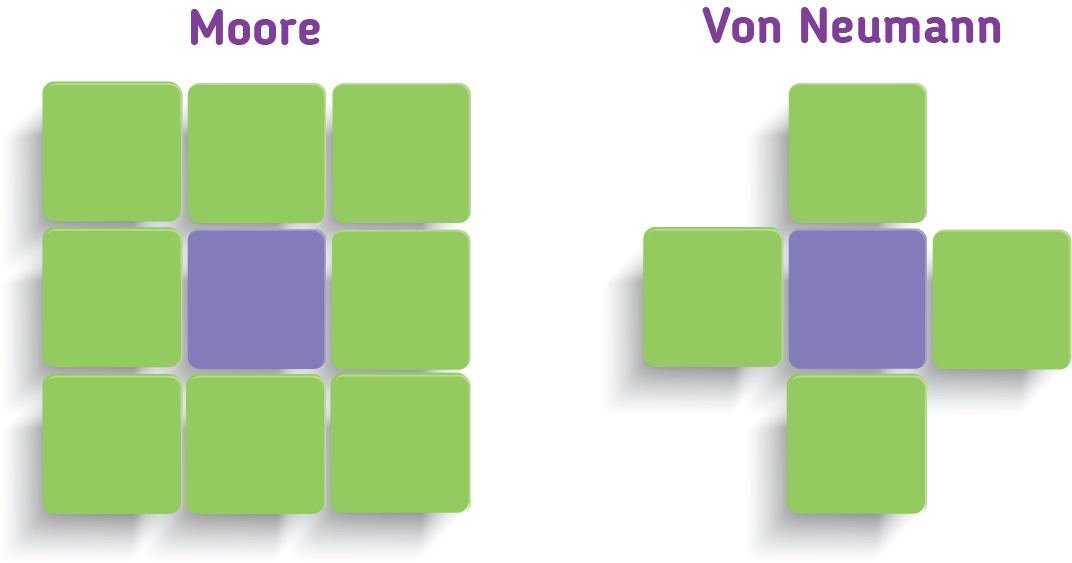
\includegraphics[width=1.0\linewidth]{EDMIIssues/Figures/sasiedztwa.png}
	\end{subfigure}
	\caption{Podstawowe typy sąsiedztwa.}
	\label{neighbours}
\end{figure} 

Budowa wszystkich komórek musi być identyczna (muszą mieć tyle samo sąsiadów, takie same zbiory stanów itp.)

Ważnym elementem konstrukcyjnym automatów komórkowych są warunki początkowe, czyli stany poszczególnych komórek w zerowej iteracji, czyli na samym początku. To od ustawienia początkowego komórek zależy dalsza ewolucja automatu, jego zachowanie, stan końcowy, tym samym powodzenie całej symulacji. Niektóre automaty komórkowe z założenia muszą mieć w odpowiedni sposób ustalone warunki początkowe

Zachowanie automatu jest definiowane m.in. poprzez warunki brzegowe, które moga być np. periodyczne, pochłaniające, czy odbijające.

Stan komórki $ x $ w chwili $ t $ oznaczmy jako $ x_t $, a stan sąsiedztwa jako $ u(x_t) $. Dla takich kryteriów stan komórki $ x $ w kolejnym kroku iteracji można opisać wzorem:\newline
$ x_{t+1} = f(u(x_t), x_t) $, gdzie:\newline
$ f $ - funkcja przejścia, która może być opisana różnego rodzaju zależnościami, np. jako tabela przejść, w postaci algorytmicznej lub jako zbiór reguł.

Po ustaleniu i zdefiniowaniu wszystkich elementów składowych automatu komórkowego można przejść do nakładania reguł na siatkę, czyli aktualizowania jej.

Podział automatów komórkowych według Wolframa:
\begin{itemize}
	\item Klasa I: Automaty niezmienne – ewoluują do czasu, kiedy wszystkie komórki osiągną identyczny stan niezależnie od stanu początkowego (zbieżne).
	\item Klasa II: Automaty ewoluujące do stanu stabilnego lub okresowych wzorców (okresowe).
	\item Klasa III: Automaty wykazujące nieporządek zarówno lokalnie, jak i globalnie, nie wykazujące żadnego wzorca (chaotyczne).
	\item Klasa IV: Automaty wykazujące bardziej złożone, długotrwałe zachowanie („żywe”).
\end{itemize}

Technika automatów komórkowych jest używana do symulacji komputerowych w wielu problemach nauki i techniki. Automaty te dostarczają również wielu zagadnień teorii dynamiki nieliniowej.

Jednym z pierwszych i najbardziej znanych przykładów automatu komórkowego jest \textit{Gra w życie} (\textit{Life}, \textit{The game of life}). Reguły tego automatu według Conwaya:
\begin{itemize}
	\item Martwa komórka, która ma dokładnie 3 żywych sąsiadów, staje się żywa w następnej jednostce czasu (rodzi się),
	\item Żywa komórka z 2 albo 3 żywymi sąsiadami pozostaje nadal żywa; przy innej liczbie sąsiadów umiera (z „samotności” albo „zatłoczenia”).
\end{itemize}
